\documentclass[10pt,aspectratio=169]{beamer}

\usetheme{metropolis}
\usepackage{amsmath,amssymb,amsfonts}
\usepackage{booktabs}
\usepackage{graphicx}
\usepackage{xcolor}
\usepackage{listings}
\usepackage{tikz}
\usetikzlibrary{positioning,shapes,arrows,fit,backgrounds,calc}

\setbeamertemplate{footline}[frame number]

\definecolor{codebg}{RGB}{245,245,245}
\definecolor{accent}{RGB}{0,122,204}
\definecolor{entropy}{RGB}{180,40,40}
\definecolor{gain}{RGB}{40,140,80}

\lstset{
  basicstyle=\ttfamily\footnotesize,
  backgroundcolor=\color{codebg},
  frame=single,
  framesep=3pt,
  xleftmargin=4pt,
  xrightmargin=4pt,
  language=C++,
  keywordstyle=\color{accent}\bfseries,
  commentstyle=\color{gray}\itshape,
  showstringspaces=false
}

\title[Trustworthiness Evaluation in CMM]{Section 4: Trustworthiness Evaluation}
\subtitle{Preventing Mismatch Errors from GNSS and Map Faults}
\author{Chenzhang Ning}
\date{2026}

\begin{document}

\frame{\titlepage}

%------------------------------------------------------------------------------
\section{Problem Motivation}
%------------------------------------------------------------------------------

\begin{frame}{The Confidence Gap in Map Matching}
  \textbf{Traditional HMM map matching} outputs only a \emph{maximum-likelihood path}.

  \vspace{0.6cm}
  \begin{columns}[T]
    \column{0.48\textwidth}
      \textbf{What we get:}
      \begin{itemize}
        \item Optimal edge sequence $E^* = (e_1, e_2, \dots, e_T)$
        \item Cumulative log-probability per node
        \item \textbf{No} per-point confidence metric
      \end{itemize}

    \column{0.48\textwidth}
      \textbf{What we need:}
      \begin{itemize}
        \item ``How certain is this match?'' — safety-critical decision
        \item ``Where did ambiguity arise?'' — root-cause diagnosis
        \item ``Is the problem GPS, map, or both?'' — feedback loop
      \end{itemize}
  \end{columns}

  \vspace{0.5cm}
  \begin{alertblock}{Core Question}
    Can we quantify \emph{epistemic uncertainty} in the matching decision at each
    epoch, using the same probabilistic framework that drove the match?
  \end{alertblock}
\end{frame}

%------------------------------------------------------------------------------

\begin{frame}{Two Complementary Trustworthiness Signals}
  CMM computes two orthogonal metrics at every epoch $t$:

  \vspace{0.4cm}
  \begin{center}
  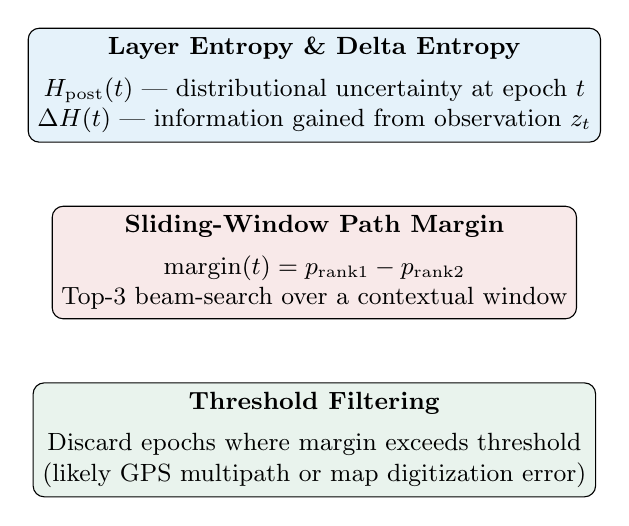
\begin{tikzpicture}[
    node distance=1.6cm,
    box/.style={draw,rounded corners,fill=white,minimum width=5.5cm,minimum height=1.3cm,align=center,font=\small},
    arrow/.style={->,>=stealth,thick,color=accent}
  ]
    \node[box,fill=accent!10] (entropy) {
      \textbf{Layer Entropy \& Delta Entropy}\\[4pt]
      $H_{\text{post}}(t)$ — distributional uncertainty at epoch $t$\\
      $\Delta H(t)$ — information gained from observation $z_t$
    };
    \node[box,fill=entropy!10,below=0.8cm of entropy] (window) {
      \textbf{Sliding-Window Path Margin}\\[4pt]
      $\text{margin}(t) = p_{\text{rank1}} - p_{\text{rank2}}$\\
      Top-3 beam-search over a contextual window
    };
    \node[box,fill=gain!10,below=0.8cm of window] (usage) {
      \textbf{Threshold Filtering}\\[4pt]
      Discard epochs where margin exceeds threshold\\
      (likely GPS multipath or map digitization error)
    };
  \end{tikzpicture}
  \end{center}

  \vspace{0.3cm}
  \begin{itemize}
    \item \textbf{Entropy} — instantaneous; \textbf{Margin} — contextual
    \item Together they distinguish \emph{local ambiguity} from \emph{path-level confusion}
  \end{itemize}
\end{frame}

%------------------------------------------------------------------------------
\section{Information Gain: Delta Entropy}
%------------------------------------------------------------------------------

\begin{frame}{Layer Entropy as Uncertainty Measure}
  For a layer with $N$ valid candidates having log-cumulative probabilities
  $\{ \ell_1, \ell_2, \dots, \ell_N \}$:

  \begin{enumerate}
    \item LogSumExp normalization (numerically stable):
    \begin{equation*}
      \ell_{\max} = \max_i \ell_i, \qquad
      S = \log\sum_i e^{\ell_i - \ell_{\max}}, \qquad
      \log p_i^{\text{norm}} = \ell_i - \ell_{\max} - S
    \end{equation*}

    \item Shannon entropy (in bits):
    \begin{equation*}
      H = -\sum_{i=1}^{N} p_i^{\text{norm}} \cdot \log_2 p_i^{\text{norm}}
    \end{equation*}
  \end{enumerate}

  \begin{itemize}
    \item $H \approx 0$: one candidate dominates — \textbf{high confidence}
    \item $H \approx \log_2 N$: uniform distribution — \textbf{maximum ambiguity}
  \end{itemize}

  \vspace{0.3cm}
  \begin{block}{Source: \texttt{cmm\_algorithm.cpp:1741-1763}}
    \begin{lstlisting}[basicstyle=\ttfamily\scriptsize]
double log_sum = log_sum_exp(layer_log_probs);
double inv_log2 = 1.0 / std::log(2.0);
for (double log_p : layer_log_probs) {
    double log_norm = log_p - log_sum;
    double p_norm = std::exp(log_norm);
    if (p_norm > 0.0) layer_entropy -= p_norm * log_norm * inv_log2;
}
    \end{lstlisting}
  \end{block}
\end{frame}

%------------------------------------------------------------------------------

\begin{frame}{Information Gain: $\Delta H = H_{\text{prior}} - H_{\text{posterior}}$}
  \textbf{Delta entropy} quantifies how much information the current GPS
  observation $z_t$ contributes to reducing uncertainty.

  \vspace{0.4cm}
  \begin{columns}[T]
    \column{0.48\textwidth}
      \textbf{First Epoch ($t=0$):}
      \begin{itemize}
        \item No prior from propagation
        \item Uniform prior: $H_{\text{prior}} = \log_2 N_{\text{valid}}$
        \item $\Delta H = \log_2 N_{\text{valid}} - H_{\text{posterior}}$
      \end{itemize}

    \column{0.48\textwidth}
      \textbf{Subsequent Epochs ($t > 0$):}
      \begin{itemize}
        \item Prior = prediction $\sum_a P(x_{t-1}=a) \cdot TP(a, b)$
        \item $H_{\text{prior}}$ from prediction log-probs
        \item $H_{\text{posterior}}$ from full $P(x_t | z_{1:t})$
      \end{itemize}
  \end{columns}

  \vspace{0.5cm}
  \begin{center}
  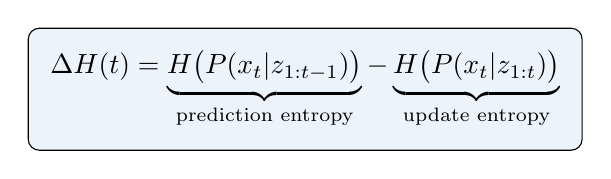
\begin{tikzpicture}
    \node[draw,rounded corners,fill=accent!8,inner sep=8pt] {
      $\Delta H(t) = \underbrace{H\big(P(x_t | z_{1:t-1})\big)}_{\text{prediction entropy}}
                     - \underbrace{H\big(P(x_t | z_{1:t})\big)}_{\text{update entropy}}$
    };
  \end{tikzpicture}
  \end{center}

  \textbf{Interpretation:}
  \begin{itemize}
    \item $\Delta H \gg 0$: observation provides strong disambiguation — \textbf{informative}
    \item $\Delta H \approx 0$: observation adds little — \textbf{redundant or noisy}
  \end{itemize}
\end{frame}

%------------------------------------------------------------------------------

\begin{frame}{Delta Entropy: First Layer Code Walkthrough}
  \begin{columns}[T]
    \column{0.55\textwidth}
      \small
      \textbf{Step 1:} Compute posterior entropy from emission-normalized cumu\_probs.

      \textbf{Step 2:} Uniform prior: $H_{\text{prior}} = \log_2(\text{valid\_count})$

      \textbf{Step 3:} Clamp $\Delta H \geq 0$ (entropy cannot decrease below zero).

    \column{0.45\textwidth}
      \begin{lstlisting}[basicstyle=\ttfamily\footnotesize,xleftmargin=2pt]
if (!layer_log_probs.empty()) {
  double H_prior = std::log2(
    static_cast<double>(
      layer_log_probs.size()));
  delta_layer_entropy =
    H_prior - layer_entropy;
  if (delta_layer_entropy < 0.0)
    delta_layer_entropy = 0.0;
}
// Assign to each node
node.delta_entropy =
  delta_layer_entropy;
      \end{lstlisting}
  \end{columns}

  \vspace{0.4cm}
  \begin{exampleblock}{Example}
    \begin{tabular}{lcc}
      \toprule
      Scenario & $N_{\text{valid}}$ & $\Delta H$ (bits) \\
      \midrule
      1 dominant candidate (99\%) & 8 & $\approx \log_2 8 = 3.0$ \\
      Uniform across 4 candidates & 4 & $\approx 0.0$ \\
      Mid confidence (top at 60\%) & 5 & $\approx 1.2$ \\
      \bottomrule
    \end{tabular}
  \end{exampleblock}
\end{frame}

%------------------------------------------------------------------------------

\begin{frame}{Delta Entropy: Subsequent Layers}
  For $t > 0$, the prior distribution is the \textbf{prediction} from the
  previous layer.

  \vspace{0.3cm}
  \begin{equation*}
    P_{\text{prior}}(x_t = b) = \frac{\sum_a P(x_{t-1}=a) \cdot TP(a,b)}
                                      {\sum_{b'} \sum_a P(x_{t-1}=a) \cdot TP(a,b')}
  \end{equation*}

  \vspace{0.3cm}
  The prediction log-probabilities are accumulated during the Viterbi
  forward pass:

  \begin{lstlisting}[basicstyle=\ttfamily\scriptsize]
// During update_layer_cmm, before multiplying by EP:
double log_sum_prev_probs = log_sum_exp(incoming_log_probs);
layer_prior_log_probs.push_back(log_sum_prev_probs);

// After the layer is complete:
node_b.cumu_prob = log_sum_prev_probs + node_b.ep; // posterior
  \end{lstlisting}

  \vspace{0.3cm}
  Then separate entropy computations on \texttt{layer\_prior\_log\_probs} and
  \texttt{layer\_log\_probs} yield $\Delta H$.

  \begin{block}{Key Insight}
    $\Delta H$ isolates the \emph{marginal contribution} of each epoch's GPS
    observation to the inference. A sudden drop signals degraded GNSS quality.
  \end{block}
\end{frame}

%------------------------------------------------------------------------------
\section{Sliding-Window Trustworthiness Margin}
%------------------------------------------------------------------------------

\begin{frame}{Why a Window-Based Metric?}
  Single-epoch entropy is \textbf{myopic}:
  \begin{itemize}
    \item A confident emission at $t$ may lead to a \emph{wrong} downstream path
    \item Ambiguity only becomes visible when considering the \emph{full sub-trajectory}
  \end{itemize}

  \vspace{0.4cm}
  \begin{center}
  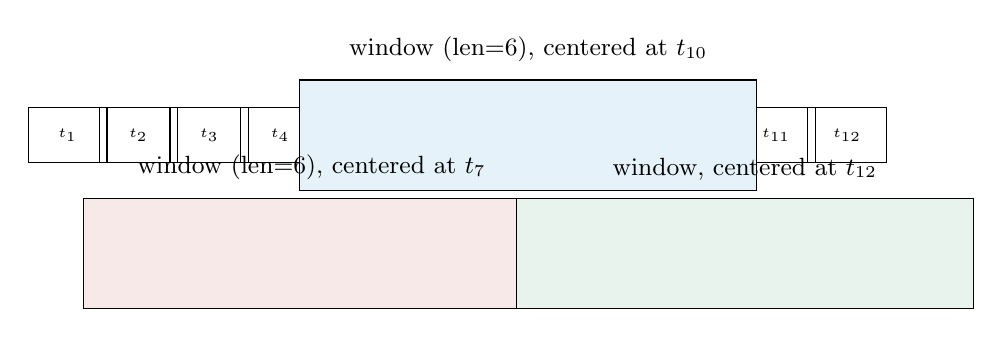
\begin{tikzpicture}[
    box/.style={draw,minimum width=1.0cm,minimum height=0.7cm,align=center,font=\tiny},
    win/.style={draw,fill=accent!10,minimum width=5.8cm,minimum height=1.4cm,align=center}
  ]
    \foreach \x in {1,2,...,12} {
      \node[box] (p\x) at (\x*0.9, 0) {$t_{\x}$};
    }
    \node[win,fit=(p5)(p6)(p7)(p8)(p9)(p10),inner sep=4pt] (w1) {};
    \node[above=0.1cm of w1,font=\small] {window (len=6), centered at $t_{10}$};

    \node[win,fit=(p2)(p3)(p4)(p5)(p6)(p7),inner sep=4pt,fill=entropy!10] (w2) at (4,-1.5) {};
    \node[above=0.1cm of w2,font=\small] {window (len=6), centered at $t_7$};

    \node[win,fit=(p8)(p9)(p10)(p11)(p12),inner sep=4pt,fill=gain!10] (w3) at (9.5,-1.5) {};
    \node[above=0.1cm of w3,font=\small] {window, centered at $t_{12}$};
  \end{tikzpicture}
  \end{center}

  \vspace{0.3cm}
  For each window $[t-k+1, t]$, compute top-$3$ independent path scores
  using \textbf{beam search}, then derive the \textbf{margin}:
  \begin{equation*}
    \text{margin}(t) = p_{\text{rank 1}} - p_{\text{rank 2}}
  \end{equation*}

  Source: \texttt{cmm\_algorithm.cpp:1801-1900}
\end{frame}

%------------------------------------------------------------------------------

\begin{frame}{Sliding-Window Algorithm Detail}
  \begin{columns}[T]
    \column{0.52\textwidth}
      \textbf{Algorithm:} \texttt{compute\_window\_trustworthiness}
      \begin{enumerate}
        \item For each end index $t \in [0, T)$:
        \item Determine start = $\max(0, t+1-\text{window\_len})$
        \item Initialize paths with emission log-probs at \texttt{start}
        \item Forward beam: propagate top-$k$ scores through each epoch
        \item At $t$: collect combined top-$k$ from all ending candidates
        \item LogSumExp normalize $\to$ linear probabilities
        \item $\text{margin} = p[0] - p[1]$
      \end{enumerate}

    \column{0.48\textwidth}
      \begin{lstlisting}[basicstyle=\ttfamily\footnotesize,xleftmargin=2pt]
// Key loop: forward pass
for (size_t cursor = start+1;
     cursor <= end_idx; ++cursor) {
  for (size_t b=0; b<tc[cursor].size(); ++b) {
    for (size_t a=0; a<tc[prev].size(); ++a) {
      double sp = get_sp_dist(...);
      if (sp < 0) continue;
      double tp = calc_tp(sp, eu);
      for (double prev_log : paths[a]) {
        push_top_k(&cur[b],
          prev_log + log(tp) + log_ep_b, 3);
}}}}

// Normalize and compute margin
double log_norm = log_sum_exp(combined);
for (double &v : combined) v = exp(v-log_norm);
if (combined.size() >= 2)
  margin = combined[0] - combined[1];
      \end{lstlisting}
  \end{columns}
\end{frame}

%------------------------------------------------------------------------------

\begin{frame}{Why Top-3? Why Beam Search?}
  \textbf{Exhaustive} enumeration over all candidate paths is $\mathcal{O}(K^W)$
  where $K \approx 8-16$ candidates and $W \approx 10$ window length.

  \vspace{0.4cm}
  \begin{columns}[T]
    \column{0.48\textwidth}
      \textbf{Top-3 Beam Search:}
      \begin{itemize}
        \item Each layer keeps only $k=3$ best cumulative log-scores per candidate
        \item $\mathcal{O}(W \cdot K^2 \cdot k)$ per window — tractable for online use
        \item Captures \emph{qualitatively distinct} alternative paths
      \end{itemize}

    \column{0.48\textwidth}
      \textbf{Why $k=3$ is sufficient:}
      \begin{itemize}
        \item $k=1$: only Viterbi — no margin
        \item $k=2$: margin available, but may miss a fundamentally different path
        \item $k=3$: balances diversity vs. computation
        \item $k > 3$: diminishing returns (exponential pruning)
      \end{itemize}
  \end{columns}

  \vspace{0.4cm}
  \begin{center}
  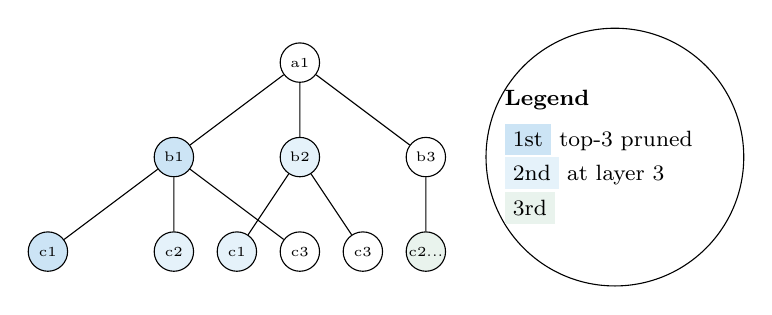
\begin{tikzpicture}[level distance=1.2cm,sibling distance=1.6cm,
    every node/.style={circle,draw,minimum size=0.5cm,font=\tiny,inner sep=0pt}]
    \node {a1}
      child { node[fill=accent!20] {b1}
        child { node[fill=accent!20] {c1} }
        child { node[fill=accent!10] {c2} }
        child { node {c3} }
      }
      child { node[fill=accent!10] {b2}
        child { node[fill=accent!10] {c1} }
        child { node {c3} }
      }
      child { node {b3}
        child { node[fill=gain!10] {c2...} }
      };
    \node[font=\footnotesize,right=0.5cm of current bounding box,text width=2.8cm] {
      \textbf{Legend}\\[4pt]
      \colorbox{accent!20}{1st} top-3 pruned\\
      \colorbox{accent!10}{2nd} at layer 3\\
      \colorbox{gain!10}{3rd}
    };
  \end{tikzpicture}
  \end{center}
\end{frame}

%------------------------------------------------------------------------------

\begin{frame}{Trustworthiness Margin in Action}
  \begin{center}
  \begin{tabular}{lcccc}
    \toprule
    Epoch & \text{rank-1 prob} & \text{rank-2 prob} & \textbf{Margin} & \text{Decision} \\
    \midrule
    $t_1$ & 0.95  & 0.03  & \textbf{0.92} & High confidence \\
    $t_2$ & 0.48  & 0.40  & \textbf{0.08} & Ambiguous — flag \\
    $t_3$ & 0.55  & 0.44  & \textbf{0.11} & Ambiguous — flag \\
    $t_4$ & 0.88  & 0.09  & \textbf{0.79} & High confidence \\
    $t_5$ & 0.35  & 0.33  & \textbf{0.02} & High ambiguity — discard \\
    \bottomrule
  \end{tabular}
  \end{center}

  \vspace{0.3cm}
  \textbf{Interpretation guidelines:}
  \begin{itemize}
    \item margin $> 0.5$: strong evidence for best path
    \item margin $\in [0.1, 0.5]$: moderate; review context
    \item margin $< 0.1$: near-tie; \textbf{likely fault} (GNSS multipath / map parallel roads)
  \end{itemize}
\end{frame}

%------------------------------------------------------------------------------
\section{Filtering \& Integration}
%------------------------------------------------------------------------------

\begin{frame}{Trustworthiness Threshold Filtering Pipeline}
  After Viterbi backtracking and window trustworthiness computation,
  a post-processing filter removes low-confidence epochs:

  \vspace{0.3cm}
  \begin{center}
  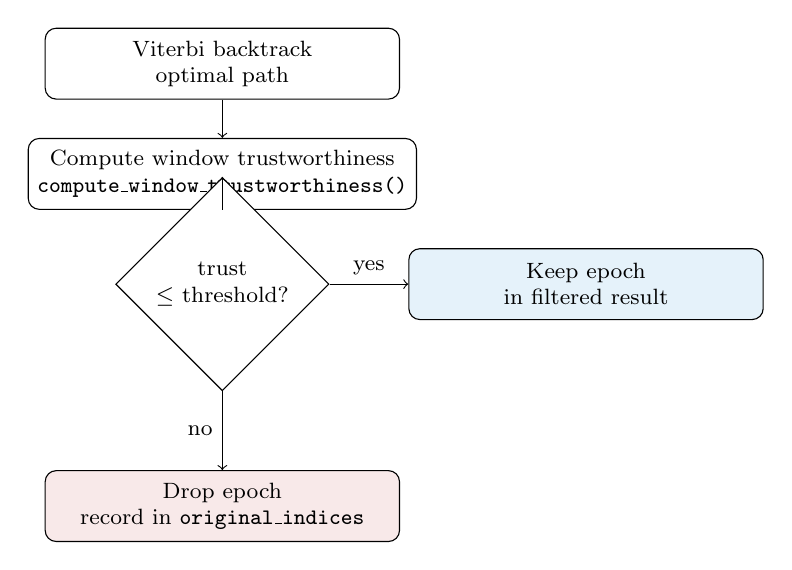
\begin{tikzpicture}[
    node distance=1.4cm,
    process/.style={draw,rounded corners,fill=white,minimum width=4.5cm,minimum height=0.9cm,align=center,font=\footnotesize},
    decision/.style={diamond,draw,fill=white,minimum width=2cm,minimum height=1cm,align=center,font=\footnotesize}
  ]
    \node[process] (viterbi) {Viterbi backtrack\\optimal path};
    \node[process,below of=viterbi] (trust) {Compute window trustworthiness\\\texttt{compute\_window\_trustworthiness()}};
    \node[decision,below of=trust] (check) {trust\\$\leq$ threshold?};
    \node[process,right=1.0cm of check,fill=accent!10] (keep) {Keep epoch\\in filtered result};
    \node[process,below=1.0cm of check,fill=entropy!10] (drop) {Drop epoch\\record in \texttt{original\_indices}};

    \draw[->] (viterbi) -- (trust);
    \draw[->] (trust) -- (check);
    \draw[->] (check) -- node[above,font=\footnotesize]{yes} (keep);
    \draw[->] (check) -- node[left,font=\footnotesize]{no} (drop);
  \end{tikzpicture}
  \end{center}

  \vspace{0.3cm}
  \begin{lstlisting}[basicstyle=\ttfamily\footnotesize]
// Source: cmm_algorithm.cpp:1315-1323
if (!config.filtered || trust <= config.trustworthiness_threshold) {
    filtered_path.push_back(mc);
    filtered_tg_opath.push_back(node);
    filtered_indices.push_back(sub_indices[i]);
}
  \end{lstlisting}
\end{frame}

%------------------------------------------------------------------------------

\begin{frame}{Output Data Model}
  \begin{columns}[T]
    \column{0.50\textwidth}
      \textbf{Per-epoch output fields:}
      \vspace{0.2cm}

      \begin{tabular}{lp{3.2cm}}
        \toprule
        Field & Description \\
        \midrule
        \texttt{trustworthiness} & Sliding-window margin\\
        \texttt{delta\_entropy}   & $\Delta H$ in bits\\
        \texttt{cumu\_prob}       & Cumulative log-prob\\
        \texttt{ep}               & Emission probability\\
        \texttt{tp}               & Normalized transition\\
        \texttt{sp\_dist}         & Shortest-path distance\\
        \bottomrule
      \end{tabular}

    \column{0.50\textwidth}
      \textbf{Per-result aggregate:}
      \vspace{0.2cm}

      \begin{tabular}{lp{3.0cm}}
        \toprule
        Field & Description \\
        \midrule
        \texttt{nbest\_trustworthiness} & Top-N scores per point\\
        \texttt{original\_indices} & Pre-filter indices\\
        \texttt{candidate\_details} & All candidate EP per point\\
        \texttt{status} & SUCCESS / PARTIAL / FAILED\\
        \bottomrule
      \end{tabular}
  \end{columns}

  \vspace{0.5cm}
  \begin{block}{Data Structure (from \texttt{mm\_type.hpp:64-72})}
    \begin{lstlisting}[basicstyle=\ttfamily\footnotesize]
struct MatchedCandidate {
    Candidate c;
    double ep;               // emission probability
    double tp;               // transition probability
    double cumu_prob;        // cumulative log-probability
    double sp_dist;          // shortest path distance
    double trustworthiness;  // window margin (CMM)
    double delta_entropy;    // information gain in bits (CMM)
};
    \end{lstlisting}
  \end{block}
\end{frame}

%------------------------------------------------------------------------------

\begin{frame}{Diagnostic Use Cases}
  \begin{columns}[T]
    \column{0.48\textwidth}
      \textbf{Case 1: Urban Canyon Multipath}
      \begin{itemize}
        \item Dense high-rises cause severe multipath
        \item GPS errors become highly anisotropic
        \item Covariance ellipse covers multiple parallel roads
        \item $\to$ \textbf{low margin} on affected epochs
        \item $\to$ \textbf{high $\Delta H$ drop} relative to open-sky segments
      \end{itemize}

    \column{0.48\textwidth}
      \textbf{Case 2: Map Digitization Error}
      \begin{itemize}
        \item Road centerline is offset from true trajectory
        \item Consistent GPS but geometric mismatch
        \item Multiple nearby edges have similar emission scores
        \item $\to$ \textbf{persistently low margin} over a segment
        \item $\to$ \textbf{moderate $\Delta H$} (no GPS anomaly)
      \end{itemize}
  \end{columns}

  \vspace{0.4cm}
  \begin{center}
  \begin{tabular}{lccc}
    \toprule
    Fault Type & Margin & $\Delta H$ & Pattern \\
    \midrule
    GPS multipath & Low (isolated) & Sharp drop & Spike \\
    GPS signal loss & Zero (multiple) & Zeros & Gap segment \\
    Map offset & Low (persistent) & Normal & Sustained \\
    Map connectivity error & Low (local) + disconnect & Normal & Junction \\
    Healthy & High ($>0.5$) & High ($>1.0$) & Stable \\
    \bottomrule
  \end{tabular}
  \end{center}
\end{frame}

%------------------------------------------------------------------------------
\section{Summary}
%------------------------------------------------------------------------------

\begin{frame}{Summary: Trustworthiness in CMM}
  \begin{enumerate}
    \item \textbf{Two complementary metrics} capture different uncertainty dimensions:
    \begin{itemize}
      \item Layer entropy / delta-entropy: \textbf{instantaneous} observation quality
      \item Sliding-window path margin: \textbf{contextual} path ambiguity
    \end{itemize}

    \item \textbf{Computationally tractable}: beam-search prevents exponential blowup
    while maintaining sufficient diversity ($k=3$ paths)

    \item \textbf{Diagnostically rich}: combinational analysis of margin + $\Delta H$
    can classify fault type (GPS vs. map vs. both)

    \item \textbf{Safety enabling}: trustworthiness thresholds allow downstream
    systems to decide confidence before acting on match results
  \end{enumerate}

  \vspace{0.4cm}
  \begin{alertblock}{Takeaway}
    CMM's trustworthiness evaluation transforms map matching from a
    \emph{black-box decision} into a \emph{quantified inference} with
    per-epoch confidence bounds — essential for safety-critical
    applications.
  \end{alertblock}
\end{frame}

%------------------------------------------------------------------------------

\begin{frame}[standout]
  \huge Questions?
\end{frame}

\end{document}
